\begin{center}
	\begin{circuitfig}[H]
		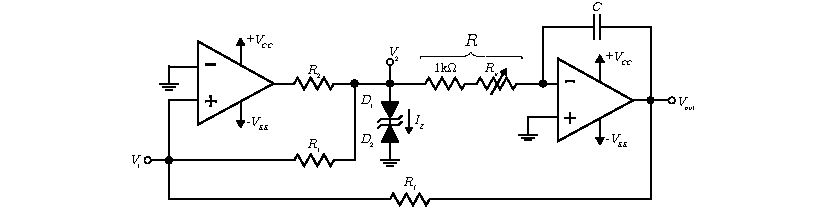
\includegraphics[width=\textwidth]{circuits/micro3_lab1.pdf}
		\caption{Γεννήτρια τριγωνικής παλμοσειράς.}
		\label{circ:1_schematic}
	\end{circuitfig}
\end{center}

Στην πρώτη άσκηση μελετάται το κύκλωμα \ref{circ:1_schematic} το οποίο αποτελείται από δύο τελεστικούς ενισχυτές 741. Για την τροφοδοσία των τελεστικών ενισχυτών είναι $V_{CC}=15\unit{\volt}$ και $V_{EE}=15\unit{\volt}$. Οι δύο δίοδοι Zener (1N750) έχουν τάση Zener $V_Z=7.5\unit{\volt}$ και τάση στην ορθή πόλωση $V_D=0.7\unit{\volt}$.\par
Βάσει των οδηγιών για την εύρεση των τιμών $R_1,R_f$ και $C$ προκύπτει $R_1=50\unit{\kilo\ohm}$, $R_1=35\unit{\kilo\ohm}$ και $C=4\unit{\nano\farad}$. Ωστόσο, επιλέχθηκαν οι πλησιέστερες τιμές που εμφανίζονται στα τυποποιημένα εξαρτήματα. Τελικα, το κύκλωμα υλοποιήθηκε με $R_1=47\unit{\kilo\ohm}$, $R_f=33\unit{\kilo\ohm}$ και $C=4.7\unit{\nano\farad}$.\par

\section{Θεωρητική μελέτη \& προσομοίωση}

	\subsection{Περιγραφή της λειτουργίας του κυκλώματος}

	\subsection{Προσομοίωση με PSpice}

	\subsection{Μέγιστη συχνότητα λειτουργίας}

	\subsection{Ρύθμιση του πλάτους τους σήματος}

\section{Εργαστηριακή εφαρμογή}

	Οι κυματομορφές $V_{\mathrm{out}}, V_1$ και $V_2$ του κυκλώματος \ref{circ:1_schematic} σε διάστημα  $1.184\unit{\milli\second}$ για $R_1=47\unit{\kilo\ohm}$, $R_2=4.7\unit{\kilo\ohm}$, $R_v=39.4\unit{\kilo\ohm}\rightarrow R=40.4\unit{\kilo\ohm}$, $R_f=33\unit{\kilo\ohm}$ και $C=4.7\unit{\nano\farad}$ δίδονται στο διάγραμμα \ref{plot:1_lab_voltages}.

	\begin{chart}[H]
		\begin{center}
			\pgfplotsset{grid style={dotted,lightgray}}
\begin{tikzpicture}
	\begin{axis}[
	grid=both,
	minor tick num=1,
	xticklabels={},
	ymin=-15,
	ymax=15,
	xtick={0,200,400,600,800,1000,1200},
	xticklabels={0,200,400,600,800,1000,1200},
	ytick={-10,-5,0,5,10},
	xlabel={Time $\(\unit{\micro\second}\)$},
	ylabel={Voltage $\(\unit{\volt}\)$}]
	\addplot+[thick,mark=none,const plot,color=DodgerBlue3]
		coordinates	{(0,0) (0,9) (0.5*592,-8) (592,9) (1.5*592,-8) (2*592,0)};
	\addplot+[thick,mark=none,domain=0:2*592,color=DeepPink3]
		coordinates {(0,6.8) (0.5*592,-7) (592,6.8) (1.5*592,-7) (2*592,6.8)};
	\addplot+[dashed,thick,mark=none,domain=0:2*592,color=black]
		coordinates {(0,0) (0,6.8) (0.5*592,0) (0.5*592,-7) (592,0) (592,6.8) (1.5*592,0) (1.5*592,-7) (2*592,0)};
	\legend{$V_2$,$V_{\mathrm{out}}$,$V_1$}
	\end{axis}
\end{tikzpicture}
			\caption{Οι τάσεις $V_1, V_2$ και $V_{\mathrm{out}}$ όπως μετρήθηκαν χρήσει του παλμογράφου στο εργαστήριο.}
			\label{plot:1_lab_voltages}
		\end{center}
	\end{chart}